\chapter{Degrees of wrongness}
\label{ch:degrees-wrongness}

The last chapter made the asterisk look crisp. A word could move out of one
part of a sentence, or it couldn't. The dependency could escape, or it was
trapped. That's part of what made syntactic islands so powerful: they made
grammar look like a map with coastlines.

But asterisks don't always feel like coastlines. Sometimes they feel like
slopes. One sentence is barely off. Another is bad, but easy to repair. A third
falls apart so badly that the intended English has to be reconstructed from
fragments.

\section{A little wrong, very wrong}

When children play, a surprising amount of the time is taken up establishing
rules: what's allowed, what's forbidden, what counts as cheating, and what
has to happen next. When my kids had friends over, I often overheard sentences
like *\mention{you're not allowed double-bouncing somebody on the
trampoline}.

That sounded wrong to me. For my English, \mention{allow} licenses a
\mention{to}-infinitival complement, as in \mention{you're allowed to bounce}.
The present participle \mention{bouncing} was off, though the neighbourhood
kids seemed perfectly happy with it.

Still, it wasn't as wrong as it could have been. Consider the sequence in
(\ref{ex:allowed-dessert}).
\ea \label{ex:allowed-dessert}
    \ea[]{\textit{You're allowed \uline{to have dessert}.}}
    \ex[\textsuperscript{?}]{\textit{You're allowed \uline{having dessert}.}}
    \ex[*]{\textit{You're allowed \uline{that you have dessert}.}}
    \ex[*]{\textit{You're allowed \uline{you have dessert}.}}
    \ex[*]{\textit{You're allowed \uline{have dessert}.}}
    \z
\z
For me, and perhaps for you too, (\ref{ex:allowed-dessert}b) is only a
little off. Example (\ref{ex:allowed-dessert}c) gets my attention.
Example (\ref{ex:allowed-dessert}d) shakes the frame more violently, and
(\ref{ex:allowed-dessert}e) falls off the cliff.

The strange thing is that each underlined piece is a possible complement
somewhere else in English.
\ea \label{ex:allowed-variants}
    \ea[]{\textit{You want \uline{to have dessert}.}}
    \ex[]{\textit{You like \uline{having dessert}.}}
    \ex[]{\textit{We told them \uline{that you have dessert}.}}
    \ex[]{\textit{We let \uline{you have dessert}.}}
    \ex[]{\textit{You can \uline{have dessert}.}}
    \z
\z
English has those forms. The verb \mention{allow} simply doesn't welcome them equally.
The wrongness comes in degrees.
% EDITORIAL-HPC: Degrees here should mean detector strength, repairability, or
% coupling strain, not degrees of membership in grammaticality. Ch. 13 should
% preserve this as graded evidence around maintained boundaries.

\section{The grammar machine}

That's not how grammaticality looks in Noam Chomsky's early generative
picture. In \textit{Syntactic Structures}, Chomsky treated grammar as a
system for generating sentences \citep{Chomsky1957}. If a string could be
generated by the grammar, it was grammatical. If it couldn't, it wasn't.

A toy grammar makes the idea concrete. Give the grammar a small lexicon,
say nouns such as \mention{dog} and \mention{cat}, determinatives such as
\mention{the} and \mention{a}, and verbs such as \mention{chases} and
\mention{sees}. Then give it rules for building noun phrases, verb phrases,
and sentences.

\begin{enumerate}
 \item N \(\rightarrow\) \{\mention{dog}, \mention{cat}\}
 \item D \(\rightarrow\) \{\mention{the}, \mention{a}\}
 \item NP \(\rightarrow\) D N
 \item V \(\rightarrow\) \{\mention{chases}, \mention{sees}\}
 \item VP \(\rightarrow\) V NP
 \item S \(\rightarrow\) NP VP
\end{enumerate}

With those rules, the grammar can build \mention{the dog chases the cat}.
Figure \ref{fig:dog-cat} shows the result.

\begin{figure}
 \centering
 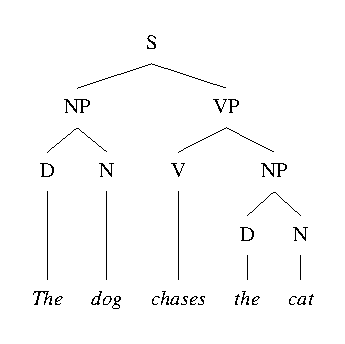
\includegraphics{figures/texstudio_wZsNnD2.pdf}
 \caption{The generated sentence \textit{The dog chases the cat}.}
 \label{fig:dog-cat}
\end{figure}

The point of the toy grammar is the clean boundary. A string generated by
the rules is in. A string not generated by the rules is out. There may be
many questions about which rules to write, but once the rules are fixed,
the answer is binary.

Computer languages give us another version of the same clean boundary. In
high school, my friend Jamie Ramsden and I spent much of computer science
class writing simple games and helping classmates with their assignments. One
assignment, perhaps a bubble sort, was due before we had left enough time for
it. We wrote one program, printed two copies, drew the required flowcharts
after the fact, and handed them in.

Our teacher, Mr. Boyko, noticed. The code was identical. That was suspicious
because even a simple program can be written in many functionally equivalent
ways. He asked whether he should give us each 50\%. We agreed this was fair,
then cheekily suggested that the same accounting should apply to the help we
had given other students. I think we both got full marks.

Computer code resembles human language in one respect: the same broad task
can be done in many ways. But a Basic interpreter isn't a human interlocutor.
If a program runs, the code is syntactically acceptable to the interpreter. It
may sort correctly, sort only some lists correctly, sort nothing correctly, or
produce useless output. Those are failures of purpose, not failures of syntax.

Human languages don't work that cleanly. A sentence can be formed from
English words in an English order and still feel more or less wrong for the
meaning, setting, speaker, or construction at hand. The asterisk marks that
failure, but it often hides how severe the failure is.

\section{More and less broken}

The easiest way to see the scale is to pile up damage. The extra stars in
(\ref{ex:dog-gradience}) are local theatre, not a standard notation. They
stand in for a feeling: some sentences are worse than others.
\ea \label{ex:dog-gradience}
 \ea[\phantom{****}]{\textit{The big black dog fetched sticks at the park.}}
 \ex[\phantom{***}\textsuperscript{?}]{\textit{The black big dog fetched sticks at the park.}}
 \ex[\phantom{***}\textsuperscript{?}]{\textit{The black big dog fetched stick at the park.}}
 \ex[\phantom{***}*]{\textit{The black big dog not fetch stick at the park.}}
 \ex[\phantom{**}**]{\textit{Black big dog no fetch stick at park.}}
 \ex[\phantom{*}***]{\textit{Black big dog no fetch park.}}
 \ex[****]{\textit{Dog big no stick no no park fetch.}}
 \z
\z
For me, the line between ordinary English and broken English falls somewhere
around (\ref{ex:dog-gradience}c) and (\ref{ex:dog-gradience}d). But that
line isn't the only thing I feel. Example (\ref{ex:dog-gradience}d) is much
closer to English than (\ref{ex:dog-gradience}g).

That may seem expected. The later examples have more things wrong with
them. In (\ref{ex:dog-gradience}c), the order of \mention{big} and
\mention{black} is unusual and \mention{sticks} has become \mention{stick}.
By (\ref{ex:dog-gradience}e), determiners are gone, \mention{not} has lost
its auxiliary, and the sentence no longer marks past tense.

So we can hold the number of errors steady. Each example in
(\ref{ex:dog-gradience2}) has just one main problem.
\ea \label{ex:dog-gradience2}
 \ea[\textsuperscript{?}]{\textit{The \uline{black big} dog fetched sticks at the park.}}
 \ex[*]{\textit{The big black dog \uline{didn't fetched} sticks at the park.}}
 \ex[*]{\textit{\uline{Big black dog} fetched sticks at the park.}}
 \ex[*]{\textit{The big black dog \uline{no fetched} sticks at the park.}}
 \ex[*]{\textit{The \uline{dog big black} fetched sticks at the park.}}
 \ex[*]{\textit{The big black dog fetched sticks at \uline{park the}.}}
 \ex[*]{\textit{The big black dog \uline{fetched sticks the park}.}}
 \ex[*]{\textit{The big black dog \uline{put sticks} at the park.}}
 \ex[*]{\textit{The big black dog fetched sticks \uline{at}.}}
 \ex[*]{\textit{The big black dog \uline{sticks at the park}.}}
 \z
\z
I've sorted these from better to worse, as best I can. You may disagree
with the order. You may even reject some of my stars. But I expect that the
set doesn't feel flat. The sentences don't all fail in the same way, with
the same force.

There's no simple hierarchy of error types here. Example
(\ref{ex:dog-gradience2}c) and example (\ref{ex:dog-gradience2}j) both
involve omissions. Example (\ref{ex:dog-gradience2}a) and example
(\ref{ex:dog-gradience2}f) both involve order. The difference seems to lie in
how much each disruption interferes with the construction we were expecting.

\section{Better and worse members}

Gradience doesn't make categories unreal. It makes them more interesting.
We already know this outside grammar. A robin is a very good bird. A penguin
is a bird too, but less central to the category most children first learn.
An ostrich is stranger still. None of that makes \term{bird} useless.

The old, classical view of categories treated membership as a matter of
necessary and sufficient conditions. A bird has feathers, lays eggs, has a
beak and wings, and lacks teeth. That works well enough until it doesn't.
Birds occasionally grow atavistic teeth. These chicks don't survive, but they
do exist, and earlier birds such as Archaeopteryx had teeth.

\begin{figure}
    \centering
    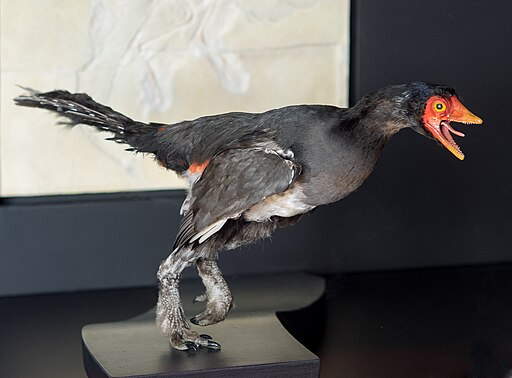
\includegraphics[width=0.8\textwidth]{figures/Archaeopteryx-Modell.jpg}
    \caption{A model of an Archaeopteryx, an early bird with teeth. Photo by Dr. Nachtigaller, CC BY-SA 4.0, \href{https://commons.wikimedia.org/wiki/File:Archaeopteryx-Modell.jpg}{via Wikimedia Commons.}}
    \label{fig:gradient-archaeopteryx}
\end{figure}

Prototype theory gives us a better way to think about this. Categories have
central members and marginal members. A marginal member isn't outside the
category simply because it's marginal. It's a worse example, not a
non-example.

The same thing happens inside grammar. \mention{Big} is a very good
adjective. It names a property, it's gradable (\mention{big},
\mention{bigger}, \mention{biggest}), and it combines with intensifiers
(\mention{very big}). It can appear before a noun, as in \mention{a big
deal}, or after a verb, as in \mention{the world is big}.

\mention{Worth} is a more awkward adjective. In \mention{it's worth your
time}, it takes something like an object, and objects normally go with verbs
and prepositions, not adjectives. You can't say *\mention{this is a
worth initiative}; you have to say \mention{worthy} or \mention{worthwhile}.
One thing isn't *\mention{worther} than another. \mention{Worth} is
still an adjective, but it lives near the edge.

That matters for grammaticality. If categories have central and marginal
members, then a sentence can be wrong because it violates a hard constraint,
because it forces a marginal member into an uncomfortable position, or because
it asks one construction to do the work of another. Those failures can feel
different.

\section{The two false exits}

Two escape routes are tempting. The first is the clean generative one: a
sentence is grammatical if the grammar generates it, and ungrammatical if it
doesn't. That view captures something real. Speakers do know patterns, and
some departures from those patterns are abrupt.

But the clean view misses the slope. It has trouble explaining why
(\ref{ex:allowed-dessert}b) feels much closer to English than
(\ref{ex:allowed-dessert}e), or why the failures in
(\ref{ex:dog-gradience2}) don't all feel equally bad.

The second escape route goes in the opposite direction. Geoffrey Sampson and
Anna Babarczy argue that the whole idea of grammaticality is misguided
\citep{Sampson2014b}. On this view, the question reduces to use: if people
produce an expression, then it belongs to the language.
% EDITORIAL-HPC: Make the anti-Sampson point projectibility-first, not just
% "speakers can make errors." Use alone fails because it doesn't tell us what
% novel cases speakers will extend, repair, or reject.

That view also captures something real. A construction may be rare, regional,
specialized, old-fashioned, playful, or new without being ungrammatical. A
sentence such as \mention{I were there} may be outside Standard English while
belonging perfectly well to another variety of English.

But use alone can't be the answer either. Speakers can produce errors. They
can quote errors, joke with errors, teach from errors, and write impossible
sentences in grammar books. We still need a way to say why
\mention{you're allowed having dessert} is easier to accept than
\mention{you're allowed have dessert}, even before we search a corpus.

\section{The slope isn't the cliff}

Gradient grammaticality is easy to overstate. The sentences don't all sit on
one smooth continuum. Several gradients are being compressed into the same
small mark.

One gradient is felt severity: how hard the sentence hits the ear. Another is
repairability: how easily we can see the intended sentence behind the one we
got. Another is category centrality: whether the words involved are being used
in ordinary or marginal ways. Another is social distribution: whether the
pattern belongs to another dialect, register, age group, profession, or
community.

Those gradients can point in different directions. A sentence may feel
unusual because it's new to us, not because it's broken. Another may be
common in casual speech and still avoided in formal prose. A third may be
easy to understand and still fail as the English we were expecting.

The asterisk hides all of this. It makes one mark do the work of several
judgments. A sentence can be more or less wrong without grammaticality
becoming unreal. Gradience is one of the ways grammar becomes visible.
% EDITORIAL-HPC: Good closing, but the synthesis chapter must cash out "visible"
% as evidence: each gradient points to a different predictor, such as severity,
% repair choice, community distribution, or context-conditioned acceptability.
